

\subsection{Problemas}
--------------------------------------------------------


\np
Una esfera metálica de radio $R$ y carga total $q$ está rodeada por un cascarón esférico metálico de radio interior $a$ y radio exterior $b$. El cascarón tiene carga neta nula. A partir de la configuración expuesta, se le pide:

\begin{figure}[H]
    \centering
    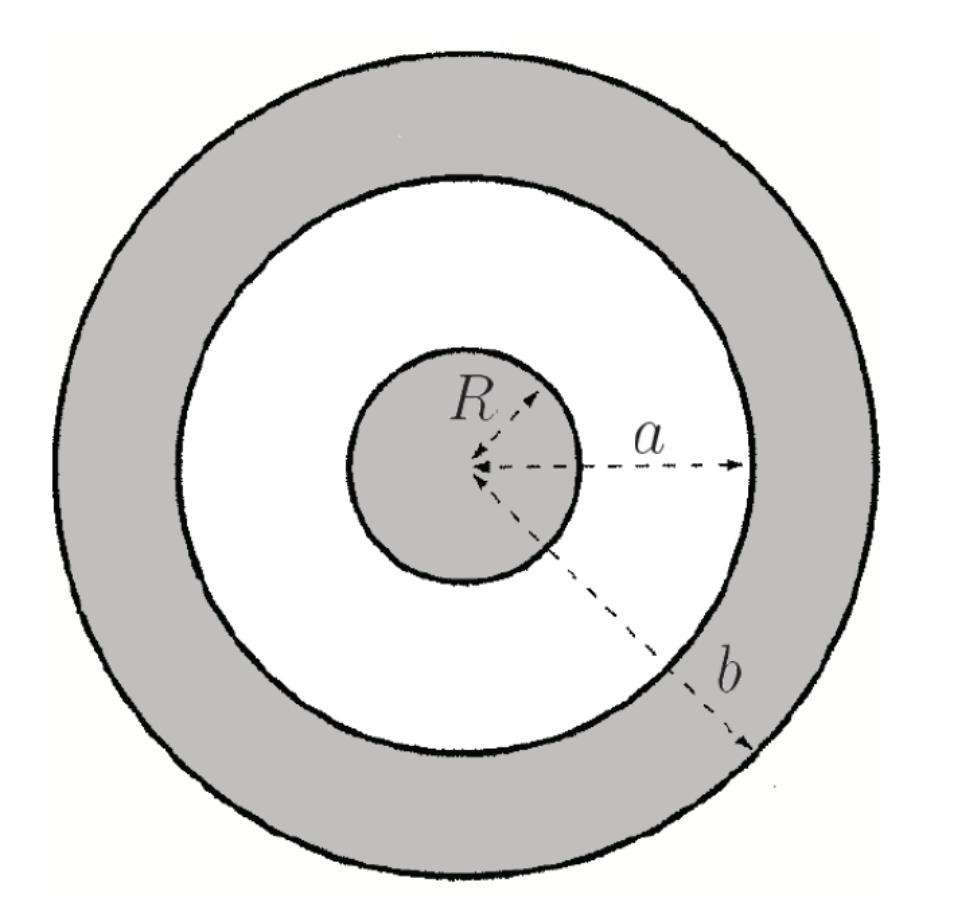
\includegraphics[width=0.6\textwidth]{Electroestática/conductores/P3G4M.jpeg}
\end{figure}

\begin{enumerate}[label=\alph*)]
    \item Encontrar la densidad superficial de carga en cada superficie
    \item Obtener el potencial eléctrico en todo el espacio.
    \item Si el cascarón exterior, se conecta a tierra, bajando su potencial a cero. ¿Cómo cambian sus respuestas anteriores?
    \item Si el cascarón exterior se conecta a un potencial V ¿Cómo cambian sus respuestas anteriores?. En este caso, ¿cuál es la carga neta en el cascarón?
    \item Suponga ahora que se conectan la esfera y el cascarón por un fino hilo conductor. En la nueva situación de equilibrio, ¿cuánto valen el campo eléctrico y el potencial en todo el espacio?
    \item Calcule la variación en la energía electrostática almacenada, como consecuencia de la conexión anterior. ¿Cómo se explica este cambio en la energía?
\end{enumerate}
\bigbreak
\bigbreak

\np
Se tiene un conductor formado por dos esferas de radios $R_1$ y $R_2$ ($R_1 < R_2$), unidas por un cable conductor de largo $L$ ($L \gg R1, R2$). Se distribuye una carga total Q en las esferas.

\begin{enumerate}[label=\alph*)]
    \item ¿Cuánta carga se va a cada esfera? ¿En cuál de las dos es mayor la carga almacenada?
    \item Calcule el potencial del alambre.
    \item ¿En cuál de las dos esferas es mayor la densidad de carga? ¿Y el campo eléctrico en la superficie?
\end{enumerate}

\begin{figure}[H]
    \centering
    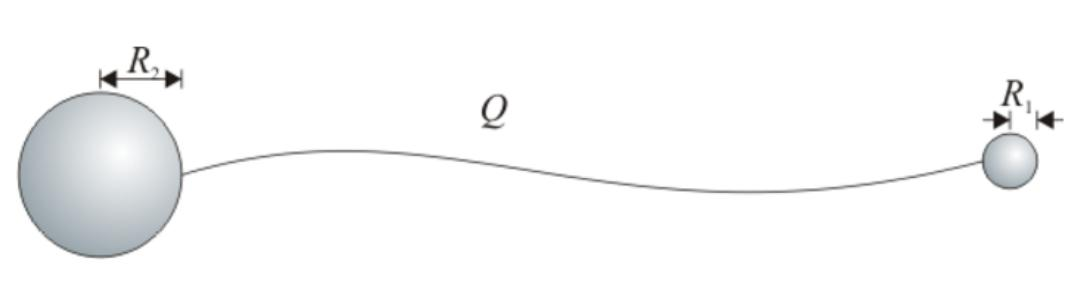
\includegraphics[width=0.7\textwidth]{Electroestática/conductores/P4G4M.jpeg}
\end{figure}
\bigbreak
\bigbreak

\np

Un condensador está hecho de tres capas esféricas concéntricas conductoras de radios $a$, $2a$ y $3a$. En lo que sigue asumiremos que las capas son lo suficientemente gruesas como para distinguir las superficies internas y externas, pero lo suficientemente delgadas como para que no necesitemos saber cuál es su grosor.
\medbreak
Las capas internas y externas están conectadas a tierra: sus potenciales se fijan en cero ($V = 0$). La capa intermedia tiene una carga neta $Q$. Esta carga induce una carga $Q_{in}$ en el borde externo de la capa interna y una carga $Q_{out}$ en el borde interno de la capa externa. Tenga en cuenta que estas cargas se toman de la tierra, por lo que los conductores interno y externo no son eléctricamente neutros.

\begin{figure}[H]
    \centering
    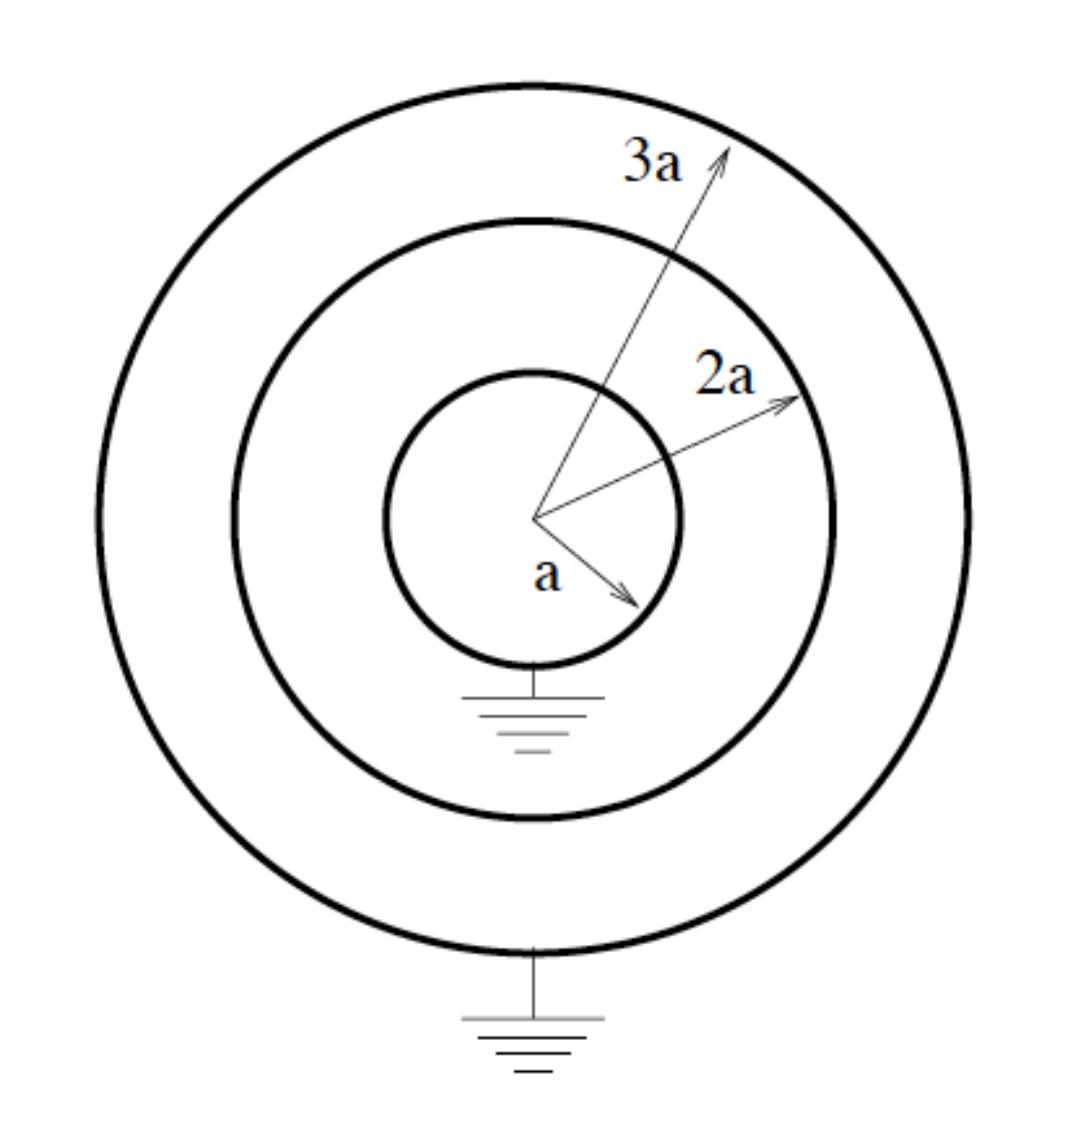
\includegraphics[width=0.6\textwidth]{Electroestática/conductores/P1G5M.jpeg}
\end{figure}

\begin{enumerate}[label=\alph*)]
    \item Calcule el campo eléctrico en todo le espacio en términos de $Q$ y $Q_{in}$.
    \item Encuentre el potencial de la capa intermedia con respecto a la tierra primero yendo de la capa interna a la capa media y luego yendo de la capa externa a la capa media.
    \item encuentre $Q_{in}$ en términos de $Q$.
    \item ¿Cuál es la energía potencial de este sistema?
    \item ¿Cuál es la capacidad de este sistema?
\end{enumerate}

\np

 Un condensador de placas paralelas de área $A$ están a una distancia $x$ entre ellas. Las dimensiones laterales de las placas son mucho más grandes que $x$.

\begin{enumerate}[label=\alph*)]
    \item El condensador se carga a un potencial $V_o$ con una batería tal que las placas se cargan con cargas $+Q$ y $-Q$. Luego, la batería se desconecta. ¿Cuánto trabajo debe realizar una fuerza externa para aumentar la separación una pequeña distancia de $x$ a $x + \Delta x$?
    \item ¿Cuál es el cambio en la energía del condensador desde el estado inicial al final? ¿Se conserva la energía?
    \item Supongamos que la batería hubiera permanecido conectada mientras la fuerza externa aumentaba la separación. ¿Cuánto trabajo realizaría la fuerza externa para aumentar la separación de $x$ a $x + \Delta x$?
    \item ¿Cuál es el cambio en la energía del condensador desde el estado inicial al final en este caso? Muestre que la energía se conserva. 
\end{enumerate}
\bigbreak
\bigbreak
\np

Considere un conductor cilíndrico largo $L$ y de radio $a$, con $L\gg a$. La carga total del cilindro es $Q$ y está distribuida uniformemente en su manto.

\begin{enumerate}[label=\alph*)]
    \item Calcule el campo eléctrico en todo el espacio.
\end{enumerate}

Considere ahora dos conductores cilíndricos de largo $L$, y de radios $a_1$ y $a_2$, separados por una distancia $d$, que es grande comparada con cualquiera de los radios, $d\gg a_1, a_2$. Las cargas totales de los cilindros son $+Q$ y $-Q$.

\begin{figure}[H]
    \centering
    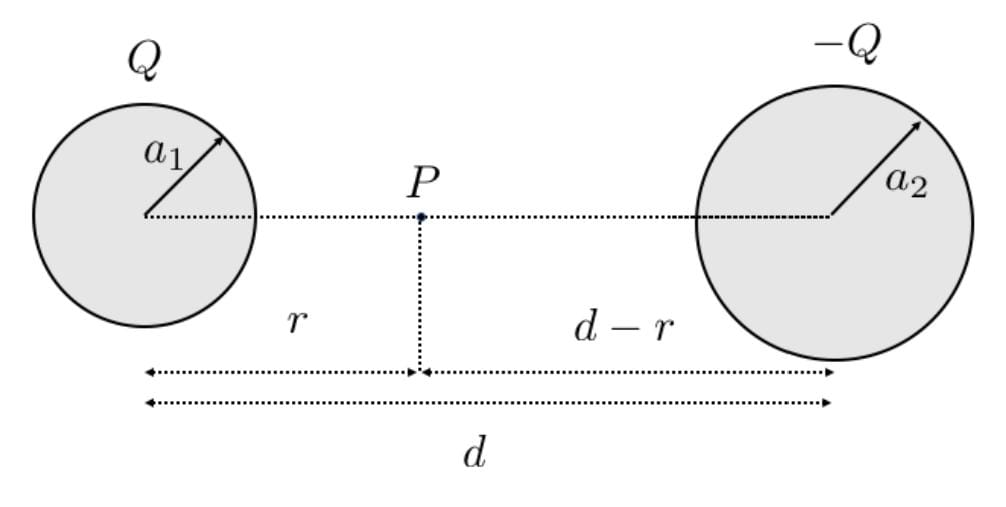
\includegraphics[width=0.6\textwidth]{Electroestática/conductores/P3G5M.jpeg}
\end{figure}

\begin{enumerate}[label=\alph*)]\setcounter{enumi}{1}
    \item Calcule el campo eléctrico en el eje que separa a ambos cilindros, es decir, en el punto $P$ de la figura.
    \item Calcule la diferencia de potencial entre ambos cilindros.
    \item Muestre que la capacitancia por unidad de largo es aproximadamente
    \[C\approx\frac{\pi\epsilon_o}{\ln\left(
    \frac{d}{\sqrt{a_1a_2}}\right)}\]
    \item Suponga que ambos conductores cilíndricos se unen por un cable conductor. Explique qué sucede, y cuál es la situación final del sistema.
\end{enumerate}
\bigbreak
\bigbreak
\np

\begin{enumerate}[label=\alph*)]
    \item Calcule la capacitancia de un condensador cilíndrico de radio interno $R_1$, radio externo $R_2$, y largo $L$.
\end{enumerate}

Ahora considere un condensador consta de tres capas cilíndricas concéntricas con radios $R$, $2R$ y $3R$. Las capas internas y externas están conectadas por un cable conductor, por lo que tienen el mismo potencial. Los conductores comienzan neutros, y luego una batería transfiere carga desde el conductor del medio a los conductores interno/externo.

\begin{enumerate}[label=\alph*)]\setcounter{enumi}{1}
    \item Si la carga final por unidad de longitud en la capa intermedia es $\lambda_b$, ¿Cuáles son las cargas por unidad de longitud en los conductores interior y exterior?
    \item ¿Cuál es la capacitancia por unidad de longitud del sistema?
    \item Si la batería se desconecta, ¿qué pasa con las tres cargas por unidad de longitud en los conductores si se agrega $\lambda_{nuevo}$ al conductor exterior?
\end{enumerate}

\newpage